\documentclass{article}
\usepackage[utf8]{inputenc}

\usepackage{listings}
\usepackage{color}
\usepackage{graphicx} %package to manage images

%New colors defined below
\definecolor{codegreen}{rgb}{0,0.6,0}
\definecolor{codegray}{rgb}{0.5,0.5,0.5}
\definecolor{codepurple}{rgb}{0.58,0,0.82}
\definecolor{backcolour}{rgb}{0.95,0.95,0.92}

%Code listing style named "mystyle"
\lstdefinestyle{mystyle}{
  backgroundcolor=\color{backcolour},   commentstyle=\color{codegreen},
  keywordstyle=\color{magenta},
  numberstyle=\tiny\color{codegray},
  stringstyle=\color{codepurple},
  basicstyle=\footnotesize,
  breakatwhitespace=false,         
  breaklines=false,                 
  captionpos=b,                    
  keepspaces=true,                 
  numbers=left,                    
  numbersep=5pt,                  
  showspaces=false,                
  showstringspaces=false,
  showtabs=false,                  
  tabsize=2
}

%"mystyle" code listing set
\lstset{style=mystyle}

\begin{document}
\centerline{\sc \large EECE 7360 Project 1}
\vspace{.5pc}
\centerline{\sc Garrett Goode and Daniel Hullihen}
\centerline{\it Spring 2017}

\section{Introduction}
The subset sum problem (also referred to as the ``exact knapsack problem'')
is defined below.

\textit{Let A = $\{a_1, ..., a_n\}$ represent some set of integers. Given a sum s, find a subset $A' \subset A$ such that
  $$s = \sum_{i=1}^n a_i, for 1 \le i \le n.$$}
In other words, if we are given a list of numbers and some target sum, we want
to find the numbers in the list that would add up to the target sum. Put as a decision
problem, the question would be ``Is there a subset A' of A where the sum of the
elements of A' is s?''

In this project, we developed a suite of instances to use as a benchmark to run
against an implementation of an exhaustive optimal algorithm for the subset
sum problem.

\section{Benchmarking}
Before any benchmark or instances can be generated, it is necessary to understand
the prior work done to evaluate implementations of algorithms that solve the
subset sum problem. The most popular metric used for determining the difficulty of
an instance of the subset sum problem is the ``density'' of the set in question.
The following equation
describes the density of a set.
$$d = n / log_2 max(a_i)$$
where n is the size of the set in quation and $max(a_i)$ is the largest element in the set.

Previous work has focused on being able to solve a
group of instances that had a some density \cite {lagarias1985}.
For example, Radziszowski and Kreher explored efficiently solving low density subset
sum problems ($d < 0.7$) \cite {kreher1988}. Schnorr and Euchner pointed out
``the hardest subset sum problems turn out to be those that
have a density that is slightly larger than 1, i.e. a density about
$1 + log_2(n/2))/n$'' \cite {schnorr94}.
On top of that, LaMacchia points out that subset sum problems with a density
$d < 0.6463...$ could be solved in polynomial time by a
``lattice oracle'' \cite {lamacchia91}, showing that there are existing algorithms
designed to work efficiently in certain areas of the instance space (in this
case, with a sufficiently low density). 

What this boils down to is: much research has focused on subset sum problems with
densities of and around 1.0. More recently, when evaluating a GPU
implementation of the subset-sum problem, Wan et al. crossed vector sizes of
36 to 54 containing random values in the range $[1, 10^8]$, covering a large
range of possible densities \cite {wan2015}. Thus, in order to provide a fair
comparison with prior work, we need to create instances with densities
on and around 1.0. For breadth, we should focus on sufficiently small and large
densities as well, and cover different combinations of set length and maximum
value that may yield the same density in order to see if those values
may have a disproprtionate impact on performance. 

\subsection{Instance Generation}
Given the prior work, when it comes to generating benchmarks for evaluating different
implementations of the subset sum problem, it is necessary to focus on the density of
the instances generated, and the range of densities covered by the overall suite.
152 instances were generated, with an emphasis on instances with densities around
1.0 in order to have a finer granularity of data. To generate each instance, we
determined the number of elements needed in the set, as well as the largest
value that will exist in the set (determined by the number of bits it represents).
For each generated number in the set, b bits of random value 0 or 1 were generated.
These bits were then concatenated together to form an interger.
Once the list was complete, we randomly chose exactly half of the elements in the
list and added them up. This sum is the solution for the instance.

The following table shows the different groups of instances that were generated
and some properties that were derived from them. In each row, a range of n and
b values were generated. These lists of values were crossed to generate
a group.
\begin{center}
  \begin{tabular}{| c | c | c | c | c | c |}
    \hline
    n (Start:End:Stride) & b (Start:End:Stride) & Count & Min d & Max d & Avg. d \\
    \hline
    2:10:2 & 20:26:2 & 20 & 0.076 & 0.5 & 0.263 \\
    \hline
    16:30:2 & 15:30:2 & 64 & 0.55 & 2.0 & 1.09 \\    
    \hline
    2:10:2 & 2:10:2 & 25 & 0.2 & 5.0 & 1.37 \\
    \hline
    50:100:10 & 15:30:5 & 24 & 1.66 & 6.66 & 3.5 \\    
    \hline
    90:100:2 & 2:10:3 & 18 & 11.25 & 50 & 26.125 \\    
    \hline
  \end{tabular}
\end{center}
Note it is possible to achieve the same density with different values of n and b.
In general, we aimed to cover a cross of large and small n with large and small b
(e.g. large set with small numbers, small set with large numbers, etc.). Together,
the above groups in the table span densities from as low as 0.076 to as high as 50,
covering a wider range than what was described in the literature. Given the emphasis
on cases around a density of 1.0, we argue this is representative of the instance
space and in line with prior work.

\section{Algorithm}
For the first attempt at solving the Subset Sum problem instances we had generated, we
chose and exhaustive "brute force" approach. Rather than attempt to target specific
subsets of our input set, we cycled iteratively through every possible solution.

\begin{lstlisting}[language=C, caption=Iterative Exhaustive Implementation]
SUBSETSUM_ALGORITHM(P1_Exhaustive)
{
    uint32_t xuwLoop;
    time_t xtStartTime, xtCurrTime;
    bool xbDone = false;

    // Clear all selections

    for(xuwLoop = 0u; xuwLoop < zptInst->suwSize; xuwLoop++)
    {
        Subset_Sum_Select(zptInst, xuwLoop, EXCLUDED);
    }

    // Start the timer

    xtStartTime = time(NULL);
    xtCurrTime = 0u;

    // The loop to find the subsets treats the inpur array 
    // elements as the digits in a binary number. This way,
    // every combination is tested as it "counts"

    while((Subset_Sum_GetSum(zptInst) != zptInst->suwTarget) &&
          (xtCurrTime < muwTimeLimit) &&
          (xbDone == false))
    {
          // Find next subset

          for(xuwLoop = 0; xuwLoop < zptInst->suwSize; xuwLoop++)
          {
              if(zptInst->saucSolution[xuwLoop] == INCLUDED)
              {
                  zptInst->saucSolution[xuwLoop] = EXCLUDED;
                  if (xuwLoop == (zptInst->suwSize - 1u))
                  {
                      xbDone = true;
                      break;
                  }
              }
              else
              {
                  zptInst->saucSolution[xuwLoop] = INCLUDED;
                  break;
              }
          }

          // Update the elapsed time

          xtCurrTime = time(NULL) - xtStartTime;
    }

}
\end{lstlisting}

As one can see in the figure above, since an element in the input set can be "in" or
"out" of the solution set, there are $2^{n}$ possible subsets. Therefore, the possible
subsets can all be represented by an n-digit binary number. In our implementation of a 
data representation of a subset sum instance, we represented a solution as an array with
the same number of elements as the input set, with each entry set to "INCLUDED" or
"EXCLUDED". This representation allowed us to emulate adding 1 to a binary number,
starting with every entry set to EXCLUDED and ending when every entry was set to INCLUDED.

Looking at the code in the preceding figure, it is easy to characterize the run time of our exhaustive algorithm.
There is an initiation step, and the $2^{n}$ possible solutions are looped through in the worst case. 
Additionally, generating the current sum of the solution set also requires cycling through all n of its elements. 
This yields the expression below.
$$O(n + n*(2^{n})) = O(2^{n})$$
As expected, the worst cases of Subset Sum cannot be solved exhaustively in poynomial time.


\section{Results}

The results are presented in the figure below. The vertical axis represents the
input size and the horizontal axis the word length of the elements in bits.

\begin{figure}[h]
\centering
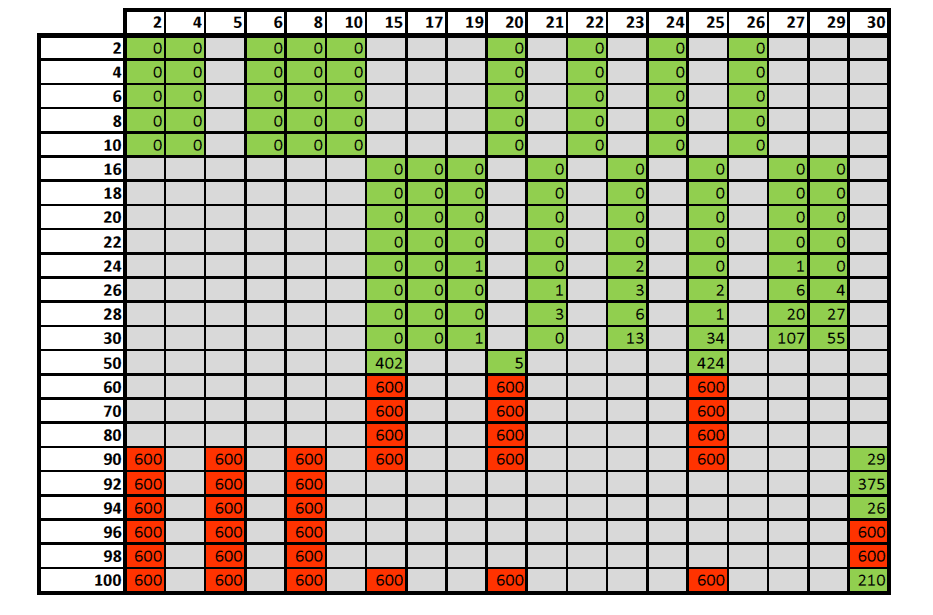
\includegraphics[width=12cm]{P1_res.png}
\caption{Run time for various input size and word length combinations}
\end{figure}

As expected, the exhaustive "brute force" approach largely failed to solve
instances where $n > 50$. This is not universally true however, as the algorithm
did manage to solve a few large instances of the largest word size we tested. From 
this we can conclude that word size does not have a large impact on the run time of
the algorithm and that brute force can be viable for even some large instances.
However speaking more generally an exhaustive approach is really only viable for
smaller instances of subset sum, per both the complexity analysis in the preceeding
section and the data presented in the last figure.

% just to generate and see the references for now


\bibliography{references}
\bibliographystyle{plain}

\end{document}
